% §8 The Three-Construction Landscape
%
% Maps the encoding space: which construction works where,
% and how the SRL conflation is resolved.

The star-tree theorem, combined with the universality of path-based
encodings (\cref{thm:tree-car}), reveals that the literature contains
three distinct encoding constructions, each with a different domain of
validity.

\subsection{Three constructions}

\paragraph{Construction~A} (index-set method, \cref{sec:index-set}):
derives index sets from a tree via~\eqref{eq:tree-derived-sets}
and applies the universal
algorithm~\eqref{eq:cj-from-scheme}--\eqref{eq:dj-from-scheme}.
\emph{Valid only for star trees} (\cref{thm:star-tree}).

\paragraph{Construction~B} (path-based method,
\cref{sec:tree-encoding}): generates Pauli strings directly from
root-to-leg paths.  \emph{Universal: valid for every encoding tree}
(\cref{thm:tree-car}).

\paragraph{Construction~F} (Fenwick-specific): the Bravyi--Kitaev
encoding uses hand-derived bit-manipulation formulas for $U$, $P$,
$\mathrm{Occ}$ that exploit the unique algebraic structure of the
Fenwick tree~\cite{fenwick1994}.  These formulas produce a correct
encoding but are \emph{not} the same as the generic tree-derived
sets of Construction~A applied to a Fenwick-shaped tree.

\subsection{Resolving the SRL conflation}

The SRL paper~\cite{seeley2012} presents JW, BK, and Parity as
instances of a single index-set framework.  On closer inspection,
this ``unification'' conflates two distinct constructions:

\begin{enumerate}
  \item \textbf{JW and Parity} are genuine Construction~A instances.
    They correspond to star trees, and their index sets are
    mechanically derivable from the generic
    formula~\eqref{eq:tree-derived-sets}.

  \item \textbf{BK} is a Construction~F instance.  Its index sets are
    hand-derived via Fenwick-tree bit arithmetic.  The SRL paper
    presents these alongside JW and Parity as if they arise from the
    same generic procedure, but they do not: BK's sets cannot be
    obtained by applying~\eqref{eq:tree-derived-sets} to the Fenwick
    tree because the Fenwick tree is not a star.
\end{enumerate}

The conflation is natural and understandable: all three encodings
\emph{can be expressed} as index-set schemes (one can always write
down the three sets for any valid encoding), and the shared language
makes them appear to be instances of a single construction.  The
distinction is in \emph{how} the sets are obtained, not \emph{what}
they are.

\subsection{The encoding landscape}
\label{sec:tree-census}

The space of $n^{n-1}$ labelled rooted trees~\cite{cayley1889}
decomposes into three construction-compatibility regions:

\paragraph{Stars ($n$ trees).}
Construction~A valid.  Trivially monotonic.  These produce relabelled
Jordan--Wigner or Parity encodings, all with $O(n)$ Pauli weight.

\paragraph{Non-star monotonic trees ($(n{-}1)! - n$ trees).}
Construction~A fails silently (well-formed operators that violate
CAR).  Construction~B valid.  The Fenwick tree is a specific member
of this class and also admits Construction~F.

\paragraph{Non-monotonic trees ($n^{n-1} - (n{-}1)!$ trees).}
Construction~A fails.  Construction~B valid.  This is the
overwhelming majority.

\begin{proposition}[Monotonic tree count]
\label{prop:monotonic-count}
The number of index-monotonic labelled rooted trees on $[n]$ is
$|M(n)| = (n{-}1)!$.
\end{proposition}

This count, verified by exhaustive enumeration for $n \le 6$
(\cref{sec:val-census}), connects encoding theory to heap-ordered
tree enumeration~\cite{bergeron1992}.

\begin{corollary}
The fraction of monotonic trees decays super-exponentially:
$(n{-}1)!/n^{n-1} \sim \sqrt{2\pi n}\;e^{-n} \to 0$.
Even if Construction~A worked for all monotonic trees (which it does
not), they would represent a vanishing minority.
\end{corollary}

Construction~B (path-based) is the only \emph{universal} method,
spanning the entire landscape.  Notably, the provably optimal encoding
(balanced ternary tree, $O(\log_3 n)$ weight) resides in the universal
class.

\subsection{Comparison of encodings}
\label{sec:encoding-comparison}

\Cref{tab:encoding-comparison} collects the key properties of the
major fermion-to-qubit encodings discussed in this paper.  Properties
include the Pauli weight (maximum number of non-identity Pauli
operators per encoded ladder operator), resource requirements, and
practical characteristics relevant to implementation.

\begin{sidewaystable*}
\caption{Comparison of fermion-to-qubit encodings for $n$ fermionic
modes.  ``Constr.''~indicates which construction produces the
encoding.  ``Max weight'' gives the worst-case Pauli weight of an
encoded ladder operator.  ``Qubits'' is the number of qubits
required.  ``Tapering'' indicates how naturally the encoding exposes
$\mathbb{Z}_2$ symmetries for qubit
tapering~\cite{bravyi2017tapering}.  ``Locality'' indicates how well
the encoding preserves spatial locality of nearest-neighbour
fermionic interactions.}
\label{tab:encoding-comparison}
\resizebox{\textwidth}{!}{%
\begin{tabular}{lccclcl}
\hline\hline
  \textbf{Encoding} & \textbf{Constr.} & \textbf{Max weight} &
  \textbf{Qubits} & \textbf{Tree shape} &
  \textbf{Tapering} & \textbf{Locality} \\
  \hline
  Jordan--Wigner~\cite{jordan1928}
    & A & $O(n)$ & $n$ & Star (chain-ordered)
    & Moderate & Excellent (1D) \\
  Parity~\cite{seeley2012}
    & A & $O(n)$ & $n$ & Star (reverse-ordered)
    & Excellent & Poor \\
  Bravyi--Kitaev~\cite{bravyi2002,seeley2012}
    & F & $O(\log_2 n)$ & $n$ & Fenwick tree
    & Moderate & Moderate \\
  Balanced binary tree~\cite{steudtner2018}
    & B & $O(\log_2 n)$ & $n$ & Balanced binary
    & Unknown & Poor \\
  Balanced ternary tree~\cite{jiang2020}
    & B & $O(\log_3 n)$ & $n$ & Balanced ternary
    & Unknown & Poor \\
  Bonsai (problem-adapted)~\cite{miller2023bonsai}
    & B & $O(\log_3 n)$ & $n$ & Optimised ternary
    & Unknown & Problem-dependent \\
  Derby--Klassen (compact)~\cite{derby2021}
    & --- & sub-$\log n$ & $< n$ & N/A
    & Unknown & Structure-dependent \\
\hline\hline
\end{tabular}%
}
\end{sidewaystable*}

Several trade-offs are visible in \cref{tab:encoding-comparison}.
Jordan--Wigner has $O(n)$ weight but preserves locality perfectly for
one-dimensional chains, making it competitive for lattice models with
near-neighbour interactions.  The Parity encoding has equally high
weight but exposes particle-number symmetries as single-qubit
operators, enabling efficient tapering~\cite{bravyi2017tapering}.  BK
achieves logarithmic weight via Construction~F, occupying a unique
niche as the only non-star tree admitting a known hand-derived
index-set encoding.  The tree-based Construction~B encodings (binary,
ternary, Bonsai) achieve the lowest weights but sacrifice locality
and have less-understood tapering properties.  The compact encodings
of Derby and Klassen~\cite{derby2021} break the $\Omega(\log n)$
barrier by relaxing the one-qubit-per-mode constraint, representing
a fundamentally different trade-off.

The ``Construction'' column makes the star-tree theorem's implications
concrete: the only standard encodings producible by the generic
index-set recipe (Construction~A) are JW and Parity, both with
$O(n)$ weight.  Every sub-linear encoding requires either
Construction~B or the unique Construction~F.

\subsection{Visual summary}

\begin{figure}[t]
\centering
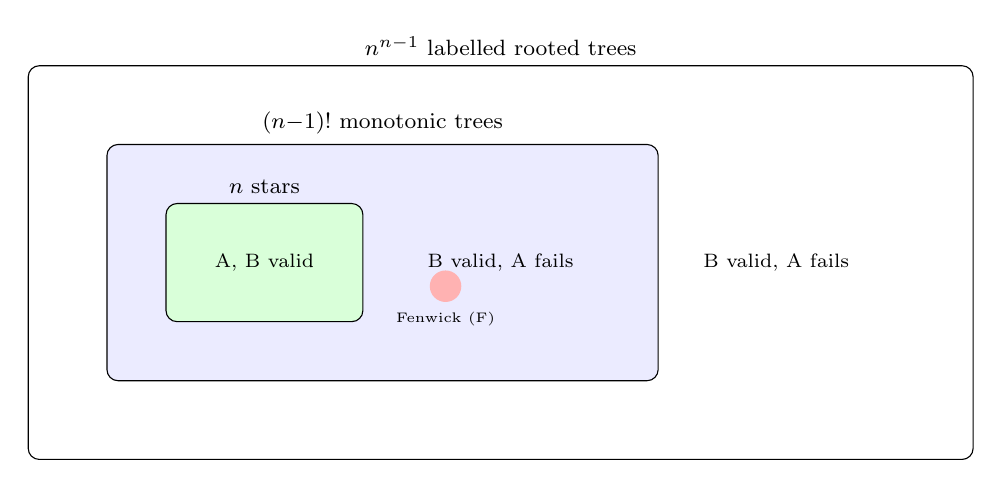
\begin{tikzpicture}[
  every node/.style={font=\small},
  region/.style={draw, rounded corners, minimum height=1.2cm, align=center}
]
  % Outer box: all trees
  \node[region, minimum width=12cm, minimum height=5cm,
    label={[font=\footnotesize]above:$n^{n-1}$ labelled rooted trees}]
    (all) {};

  % Middle box: monotonic trees
  \node[region, minimum width=7cm, minimum height=3cm,
    fill=blue!8,
    label={[font=\footnotesize]above:$(n{-}1)!$ monotonic trees}]
    at ([xshift=-1.5cm]all.center) (mono) {};

  % Inner box: stars
  \node[region, minimum width=2.5cm, minimum height=1.5cm,
    fill=green!15,
    label={[font=\footnotesize]above:$n$ stars}]
    at ([xshift=-1.5cm]mono.center) (stars) {};

  % Labels
  \node[font=\scriptsize] at (stars.center) {A, B valid};
  \node[font=\scriptsize, align=center] at ([xshift=1.5cm]mono.center) {B valid, A fails};
  \node[font=\scriptsize, align=center] at ([xshift=3.5cm]all.center) {B valid, A fails};

  % Fenwick tree marker
  \node[circle, fill=red!30, minimum size=0.4cm, inner sep=0pt,
    label={[font=\tiny]below:Fenwick (F)}]
    at ([xshift=0.8cm, yshift=-0.3cm]mono.center) {};
\end{tikzpicture}
\caption{The three-construction landscape.  Stars (green) are the only
trees where Construction~A produces valid encodings.  The Fenwick tree
(red dot) lies in the monotonic region and also admits Construction~F.
Construction~B works everywhere.}
\label{fig:landscape}
\end{figure}
